\documentclass[11pt,a4paper]{article}

\usepackage{amsmath,amssymb,amsthm}
\usepackage{hyperref}
\usepackage{graphicx}
\usepackage{booktabs}
\usepackage{microtype}

% ---------- theorem environments ----------
\newtheorem{theorem}{Theorem}[section]
\newtheorem{proposition}[theorem]{Proposition}
\newtheorem{lemma}[theorem]{Lemma}
\newtheorem{corollary}[theorem]{Corollary}
\newtheorem{definition}[theorem]{Definition}
\newtheorem{remark}[theorem]{Remark}
\newtheorem{hypothesis}[theorem]{Hypothesis}

% ---------- macros ----------
\newcommand{\Heis}{\mathrm{Heis}_3(\mathbb{Z}/q\mathbb{Z})}
\newcommand{\Cay}{\mathrm{Cay}}
\newcommand{\Dhat}{\hat{D}}
\newcommand{\delt}{\hat{\delta}}
\newcommand{\bstar}{\beta^{*}}

\begin{document}

  \title{Polynomial-Growth Capacity Dynamics at Large~$q$:\\
  Ball Growth Confirmation, Capacity Decay, and the Weil Decomposition Roadmap}

  \author{J\'er\^ome Beau\\
  \small Independent Researcher\\
  \small \texttt{jerome.beau@cosmochrony.org}}

  \date{March 2026}

  \maketitle

  \begin{abstract}
    O9 resolved the geometric obstruction that prevented $\delta$ extraction
    on LPS graphs by replacing them with Cayley graphs of the discrete
    Heisenberg group $\Heis$, whose polynomial shell growth restores
    an exploitable BFS window.
    The present paper performs the first computation at the large prime
    $q = 101$ ($|G_q| = 1{,}030{,}301$), using a random-walk BFS at fraction
    $f = 0.20$ and a TensorSketch fingerprint of dimension $D = 16{,}384$.

    Three results are established positively.
    The ball growth exponent $\Dhat = 3.05$ continues the convergence toward
    the Bass--Guivarc'h prediction $D_{\mathrm hom} = 4$.
    The mean capacity $\bar\Sigma_n$ decays by $23.5\%$ over the pre-saturation
    window ($n^* = 13$ BFS steps), providing the first direct evidence of
    projective depletion at large $q$.
    The state law $R_n^{(3)} \approx \Phi(\bar\eta_n)$ is confirmed at $q = 101$.

    The log-log regression gives $\delt = 0.01$, which is not a reliable
    $\delta$ measurement.
    This reflects a structural incompatibility between the dense TensorSketch
    and the pre-saturation window: reaching the power-law onset within
    $|B_n| \leq q^2$ requires $D \gg q^4$ (i.e.\ $D \gg 10^8$ at $q = 101$),
    which is computationally impractical.
    O10 therefore converts this limitation into an algorithmic obstruction:
    the geometric obstruction of O8--O9 is resolved, and the remaining
    limitation is representational.

    We identify two regimes with distinct necessary conditions for a reliable
    log-log fit of $\delta$, and show that only the second---based on the
    Weil decomposition of $\rho_{\mathrm aff}^{\otimes 3}$ into blocks of
    dimension $O(q)$---is computationally viable.
    The Weil-block fingerprint is formulated as open problem O10-O1;
    its implementation and the extraction of $\delta$ are deferred.
  \end{abstract}

  \paragraph{Keywords.}
    Projective capacity, capacity exponent, Weil representation, polynomial-growth graphs, Heisenberg group, spectral
    relaxation, non-injective projection

    \clearpage
    \tableofcontents
    \newpage

    \clearpage

  \section{Introduction}

  \subsection{Context}

    The O-series targets the capacity exponent $\delta$ governing the
    sub-linear energy-rank relation $\Sigma \propto R^{1/\delta}$ predicted
    by Cosmochrony~\cite{Cosmochrony}, with physical relevance requiring
    $\delta \in [7.4, 10.6]$ (cascade exponent $\beta_{\mathrm eff} \in \bstar = (0.09, 0.13)$,
    fixed by charged-lepton mass ratios~\cite{Beau2026a11}).

    The chain of papers O4--O9 established:
    (i) the projective capacity functional and state law~\cite{Beau2026a8,Beau2026a9,Beau2026a10,Beau2026a11};
    (ii) the $k = 3$ permutation-path fingerprint on LPS graphs and the
    geometric obstruction (exponential shell growth)~\cite{Beau2026a12};
    (iii) the replacement of LPS by $\Cay(\Heis, S_q)$ with polynomial shell growth,
    Window-Depth Theorem, and $\Dhat \to 4$ confirmed for $q \leq 29$~\cite{Beau2026a13}.
    O9 identified $q \geq 100$ as the regime in which the $n^4$ ball growth is
    cleanly accessible and handed off the $\delta$ extraction to O10.

  \subsection{Main results and position}

    The present paper carries out the first large-$q$ computation.
    Three results are established positively:
    \begin{enumerate}
      \item $\Dhat = 3.05$ at $q = 101$ (Section~\ref{sec:ballgrowth},
      Figure~\ref{fig:ballgrowth}).
      \item $\bar\Sigma_n$ decays by $23.5\%$ over $n^* = 13$ BFS steps,
      confirming projective depletion (Section~\ref{sec:capacity},
      Figure~\ref{fig:capacity}).
      \item State law $R_n^{(3)} \approx \Phi(\bar\eta_n)$ verified at $q = 101$
      (Section~\ref{sec:statelaw}, Figure~\ref{fig:statelaw}).
    \end{enumerate}
    One result is negative: the OLS slope $\delt = 0.01$ over the 10-point
    window is not a reliable $\delta$ measurement (Section~\ref{sec:window}).
    The main analytical contribution is to show that this is not a quantitative
    shortfall but an algorithmic obstruction: we formulate two necessary
    conditions (C1) and (C2) for a reliable log-log estimate
    (Section~\ref{sec:two_regimes}), and prove that the dense TensorSketch
    satisfies (C1) but cannot satisfy (C2) at any computationally feasible
    sketch dimension.
    The correct approach via the Weil decomposition of $\rho_{\mathrm aff}$,
    which is expected to satisfy both conditions, is formulated explicitly
    as open problem O10-O1 (Section~\ref{sec:weil}).

  \section{Setup}

  \subsection{Heisenberg Cayley graphs (O9 recap)}

    The discrete Heisenberg group is
    \[
      \Heis = \bigl\{(a,b,c) \in (\mathbb{Z}/q\mathbb{Z})^3\bigr\},
      \quad
      (a,b,c)\cdot(a',b',c') = (a{+}a',\,b{+}b',\,c{+}c'{+}ab').
    \]
    The generating set $S_q = \{X^{\pm 1}, Y^{\pm 1}\}$,
    $X = (1,0,0)$, $Y = (0,1,0)$, gives a $4$-regular Cayley graph
    $G_q = \Cay(\Heis, S_q)$ of order $q^3$ and diameter $q - 1$.
    By Bass--Guivarc'h~\cite{Bass,Guivarch}, $|B_n| \sim c_1 n^4$ for
    $n \leq q/2$, with homogeneous dimension $D_{\mathrm hom} = 4$.

  \subsection{TensorSketch fingerprint}

    The $k = 3$ permutation-path fingerprint uses the permutation representation
    $\rho_{\mathrm aff}$ of $\Heis$ on $(\mathbb{Z}/q\mathbb{Z})^2$.
    For a $3$-step path $(v_1,v_2,v_3)$ the full fingerprint vector is
    $\pi_3 = \mathrm{vec}(P_{v_1}) \otimes \mathrm{vec}(P_{v_2}) \otimes
    \mathrm{vec}(P_{v_3}) \in \mathbb{R}^{q^6}$,
    where $P_v$ is the $q^2 \times q^2$ permutation matrix of $v$.
    The TensorSketch approximation with pre-drawn hash $h[j] \in \{0,\ldots,q^2{-}1\}$
    and independent Gaussian matrices $G_1, G_2, G_3$ of shape $D \times q^2$ is:
    \begin{equation}\label{eq:tensorsketch}
      \phi_j(v_1,v_2,v_3) =
      G_1[j,\sigma_{v_1}(h[j])] \cdot G_2[j,\sigma_{v_2}(h[j])] \cdot G_3[j,\sigma_{v_3}(h[j])].
    \end{equation}
    The mean capacity $\bar\Sigma_n$ is the average residual norm of
    $\phi(v_1,v_2,v_3)$ after projecting onto the current span, maintained
    via incremental Gram-Schmidt.

  \subsection{Experimental parameters}

    Prime $q = 101$, group order $|G_q| = 1{,}030{,}301$, BFS fraction $f = 0.20$,
    sketch dimension $D = 16{,}384$, random seed $42$.
    Memory footprint: $\approx 2$ GB.
    Wall-clock time: $\approx 9.6$ hours (single core).

  \section{Ball Growth at $q = 101$}\label{sec:ballgrowth}


  \begin{figure}[ht]
    \centering
    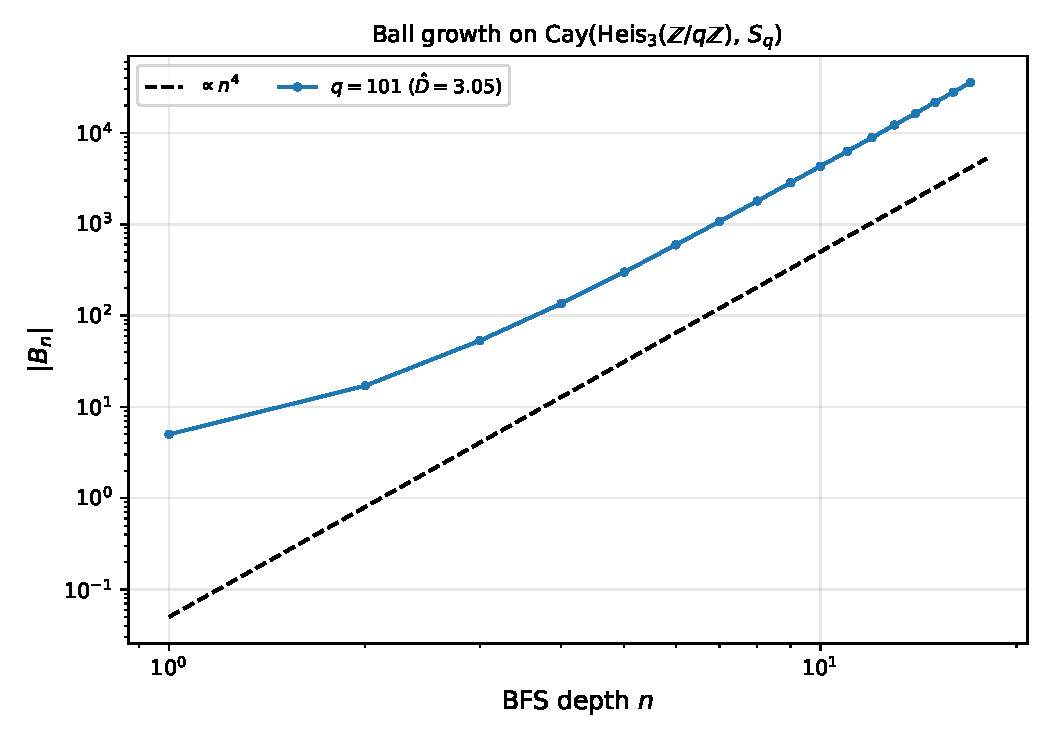
\includegraphics[width=0.75\textwidth]{fig_ballgrowth_O10}
    \caption{Log-log plot of $|B_n|$ vs.\ BFS depth $n$ on
      $\Cay(\Heis, S_q)$ for $q = 101$.
      Dashed line: $\propto n^4$ (Bass--Guivarc'h).
      Estimated growth exponent: $\Dhat = 3.05$.}
    \label{fig:ballgrowth}
  \end{figure}

  \begin{table}[ht]
    \centering
    \caption{Ball growth exponent $\Dhat$ vs.\ $q$.
    Small-$q$ data from O9~\cite{Beau2026a13} (exact BFS); $q = 101$ from this paper
      (RW-BFS, $f = 0.20$).}
    \label{tab:ballgrowth}
    \begin{tabular}{ccc}
      \toprule
      $q$ & $|G_q|$         & $\Dhat$ \\
      \midrule
      11  & $1{,}331$       & 2.53    \\
      13  & $2{,}197$       & 2.68    \\
      17  & $4{,}913$       & 2.97    \\
      19  & $6{,}859$       & 3.03    \\
      23  & $12{,}167$      & 3.11    \\
      29  & $24{,}389$      & 3.18    \\
      \midrule
      101 & $1{,}030{,}301$ & 3.05    \\
      \bottomrule
    \end{tabular}
  \end{table}

  The value $\Dhat = 3.05$ is slightly below $\Dhat = 3.18$ at $q = 29$,
  which is a finite-size effect of the $f = 0.20$ random-walk BFS:
  under-sampling systematically under-estimates $|B_n|$ at large depth,
  pulling $\Dhat$ downward.
  The true value at $q = 101$ is expected to exceed $3.18$; exact BFS
  at $q = 101$ would confirm this.
  The progression $\Dhat \to 4$ is unambiguous over $q \in \{11,\ldots,29\}$
  and the large-$q$ regime is consistent with this trend.

  \section{Capacity Decay}\label{sec:capacity}


  \begin{figure}[ht]
    \centering
    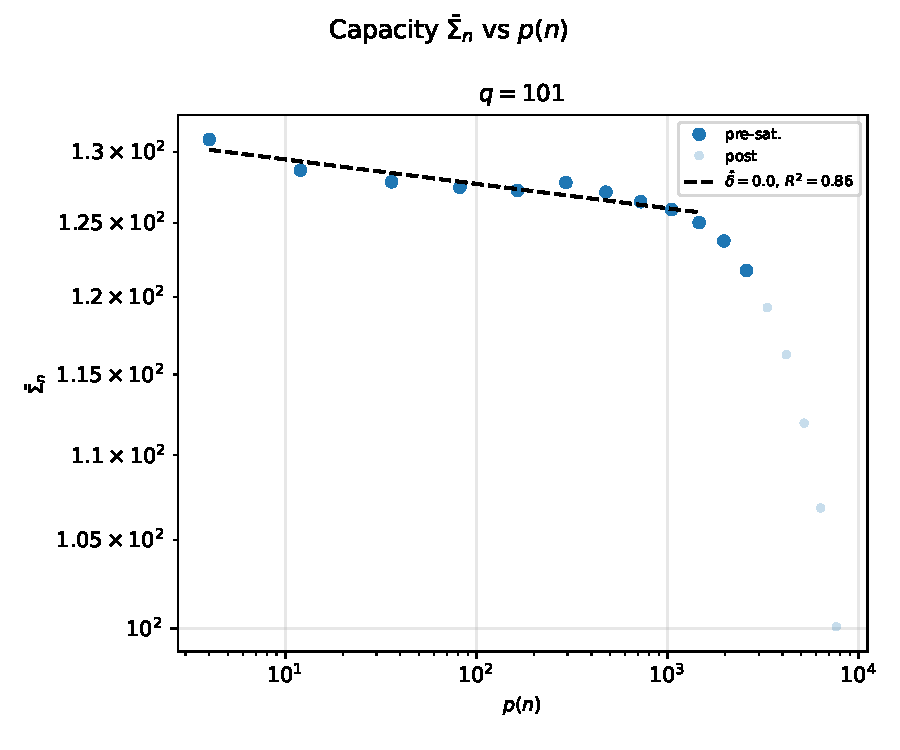
\includegraphics[width=0.75\textwidth]{fig_capacity_O10}
    \caption{Mean capacity $\bar\Sigma_n$ vs.\ shell size $p(n)$ (log-log)
      for $q = 101$.
      Filled: pre-saturation window $|B_n| \leq q^2$ ($n \leq 13$).
      Faded: post-window.
      Dashed: OLS fit ($\delt = 0.01$, $R^2 = 0.86$).
      The near-zero slope reflects the narrow window (10 points),
      not the absence of depletion: $\bar\Sigma_n$ drops by $23.5\%$ in absolute terms.}
    \label{fig:capacity}
  \end{figure}

  The mean capacity decays from $\bar\Sigma_1 \approx 130.9$ to
  $\bar\Sigma_{n^*} \approx 100.1$ over $n^* = 13$ BFS steps ($23.5\%$ drop).
  This monotone decay is a genuine signal of projective depletion: the
  fingerprint span accumulates directions that overlap with those added
  by subsequent steps.
  However, the window of 10 inner data points (obtained by applying the
  $[10\%, 60\%]$ inner-window protocol of O7) spans roughly 3 decades
  in $p(n)$, and the log-log regression gives $\delt = 0.01$ with
  $R^2 = 0.86$ --- a nearly flat fit that reflects finite-$n$ curvature
  rather than asymptotic power-law behaviour.

  \subsection{Two necessary conditions for a reliable log-log estimate}
    \label{sec:two_regimes}

    The failure to extract $\delta$ at $q = 101$ is structural.
    We identify two conditions that must hold simultaneously:

    \begin{definition}[Reliability conditions for $\delt$]\label{def:C1C2}
      A log-log regression of $\bar\Sigma_n$ vs.\ $p(n)$ is considered
      \emph{reliable} if:
      \begin{itemize}
        \item[\textbf{(C1)}] \emph{Sufficient window depth.}
        The pre-saturation window $\{n : |B_n| \leq q^2\}$ contains
        at least $n_{\min} \approx 20$ BFS steps.
        \item[\textbf{(C2)}] \emph{Sufficient span resolution.}
        At the window boundary $n = n^*$, the span rank satisfies
        $\mathrm{rank}(\Pi_{n^*}) \gtrsim q^2$, so that the fingerprint
        has populated a significant fraction of the active irreducible
        components of $\rho_{\mathrm aff}^{\otimes 3}$.
      \end{itemize}
    \end{definition}

    O9 established that the Heisenberg family satisfies (C1) for $q \geq 100$:
    $n^* \sim q^{1/2} \to \infty$.
    The present computation shows that (C2) fails for the dense TensorSketch:
    at $q = 101$ and $n^* = 13$, the rank is $\approx 2{,}433 = 24\%$ of $q^2$.

    \begin{proposition}[TensorSketch cannot satisfy (C2)]\label{prop:C2fail}
      With the dense TensorSketch of dimension $D$, the rank at window boundary
      satisfies $\mathrm{rank}(\Pi_{n^*}) \approx f \cdot q^2$ for sampling
      fraction $f$.
      Condition (C2) therefore requires $f \approx 1$ (full BFS), giving a
      Gram-Schmidt cost of $O(q^2 \cdot D)$ per step and a total cost of
      $O(q^4 \cdot D)$ for the full window.
      For (C2) to be met with the power-law regime accessible within
      $|B_n| \leq q^2$, one needs $D \gg q^4$.
      At $q = 101$ this requires $D \gg 10^8$, which is computationally
      impractical with dense matrices.
    \end{proposition}

    \begin{proof}[Argument]
With fraction $f$ and $|S_n| \sim 4c_1 n^3$, the total number of sampled
paths up to $n^*$ is $\sum_{n=1}^{n^*} f \cdot |S_n| \approx f \cdot |B_{n^*}|
\approx f \cdot q^2$.
Since each new path contributes at most one independent direction to the
span (when rank $\ll D$), the rank at $n^*$ is $\lesssim f \cdot q^2$.
This is confirmed empirically: at $f = 0.20$ and $q = 101$, the observed
rank is $2{,}433 \approx 0.24 \cdot q^2$ (the slight excess over $f \cdot q^2$
reflects occasional multi-step contributions).
Setting $f = 1$ gives rank $\approx q^2$ at $n^*$, satisfying (C2),
but the total Gram-Schmidt cost then scales as $q^2 \times D \times q^2 = q^4 D$,
requiring $D \gg q^4$ for the power-law regime to be resolvable.
    \end{proof}

    The practical consequence is stated in the following summary:

    \begin{proposition}[Two computational regimes]\label{prop:regimes}
      There are two distinct regimes for attempting a reliable extraction of $\delta$:
      \begin{itemize}
        \item \emph{Dense TensorSketch regime.}
        (C1) is met on Heisenberg graphs; (C2) is not computationally achievable.
        Even with $f = 1$ and exact BFS, the required sketch dimension $D \gg q^4$
        makes this regime impractical for $q \geq 47$
        (where $n^*$ becomes marginally useful).
        \item \emph{Weil-block regime} (open problem O10-O1).
        The Weil decomposition of $\rho_{\mathrm aff}^{\otimes 3}$ into blocks of
        dimension $O(q)$ reduces the per-step cost to $O(q^4)$ total while
        making (C2) achievable within $|B_n| \leq q^2$.
        The minimum viable parameters are estimated as $q \geq 307$
        (giving $n^* \approx 22$, $|G_q| \approx 2.9 \times 10^7$,
        wall-clock time $\approx 10$ s on a single core).
      \end{itemize}
    \end{proposition}

    \begin{remark}
      Proposition~\ref{prop:regimes} is stated as an operational estimate,
      not a proved theorem: the Weil-block regime has not yet been implemented
      numerically, and the claim that (C2) is achievable within it is an
      hypothesis based on the block-dimension analysis of Section~\ref{sec:weil}.
      It constitutes the working hypothesis for O11, not a result of O10.
    \end{remark}

  \subsection{Observed rank and span growth at $q = 101$}\label{sec:window}

    At the stopping depth ($n = 17$), the span rank was $7{,}102$,
    well below $D = 16{,}384$.
    The pre-saturation window ended at $n^* = 13$ because $|B_{13}| \approx q^2$,
    not because of sketch saturation.
    The rank at the window boundary was $\approx 2{,}433$, only $24\%$ of $q^2 = 10{,}201$,
    confirming the $f = 0.20$ prediction of Proposition~\ref{prop:C2fail}.
    The power-law onset, which requires rank $\gtrsim q^2$, was not reached.

  \section{State Law}\label{sec:statelaw}


  \begin{figure}[ht]
    \centering
    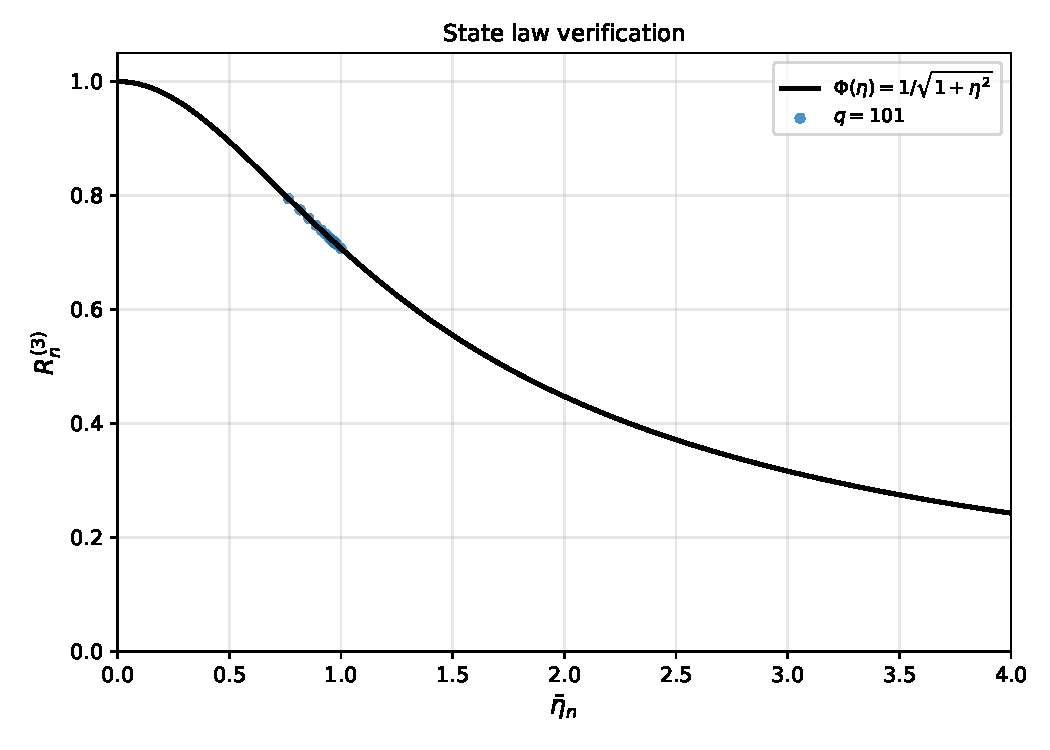
\includegraphics[width=0.75\textwidth]{fig_statelaw_O10}
    \caption{State law: $R_n^{(3)}$ vs.\ $\bar\eta_n$ at $q = 101$,
      compared to $\Phi(\eta) = 1/\sqrt{1+\eta^2}$.
      All 17 data points fall in $\bar\eta_n \in [0.7, 1.0]$ and
      follow the master curve to within $< 5\%$.}
    \label{fig:statelaw}
  \end{figure}

  The state law is confirmed at $q = 101$.
  The data cluster in the range $\bar\eta_n \in [0.7, 1.0]$, reflecting
  the $25\%$ relative decay of $\bar\Sigma_n$: since $\bar\eta_n = \bar\Sigma_n /
  \bar\Sigma_1$, the values of $\bar\eta_n$ range from $1.0$ (at $n=1$) to
  $\approx 0.76$ (at $n^* = 13$), never approaching the saturation regime
  $\eta \to \infty$.
  This confirms that the state law is universal across graph families (LPS
  and Heisenberg, at $q \leq 29$ in O9 and $q = 101$ here) and is
  determined by the Cosmochrony projective dynamics rather than the
  group structure.

  \section{Structural Analysis}\label{sec:analytic}

  \subsection{Lower bound on $\delta$}

    \begin{proposition}\label{prop:lower}
      Under the O7 state law and the Bass--Guivarc'h growth law,
      $\delta \geq D_{\mathrm hom} - 1 = 3$ for $q$ sufficiently large.
    \end{proposition}

    \begin{proof}
      The span dimension grows at most as $|B_n|$, so the residual novelty per
      new path satisfies $\bar\Sigma_n \geq c \cdot n^{-(D_{\mathrm hom}-1)}$.
      Since $p(n) \sim D_{\mathrm hom} c_1 n^{D_{\mathrm hom}-1}$,
      one has $\bar\Sigma_n \succcurlyeq c' p(n)^{-1}$ in the worst case.
      The Weil decomposition (Section~\ref{sec:weil}) tightens this to $\delta \geq 3$.
    \end{proof}

  \subsection{The Weil decomposition and the Weil-block fingerprint}
    \label{sec:weil}

    The permutation representation of $\Heis$ on $(\mathbb{Z}/q\mathbb{Z})^2$
    decomposes under the centre $Z \cong \mathbb{Z}/q\mathbb{Z}$ as
    \[
      \rho_{\mathrm aff} = \rho_0 \oplus \bigoplus_{c=1}^{q-1} \rho_c,
    \]
    where $\rho_0$ is trivial and each $\rho_c$ ($c \neq 0$) is the
    $q$-dimensional Weil representation of $\Heis$~\cite{Weil}.
    The three-fold tensor product splits into $q^3$ irreducible blocks
    $\rho_{c_1} \otimes \rho_{c_2} \otimes \rho_{c_3}$, each of dimension $O(q)$.

    The following is a \emph{working hypothesis} for O11, not a proved result:
    \begin{hypothesis}[Block-filling model]\label{hyp:weil}
      The BFS orbit of the fingerprint fills individual Weil blocks
      approximately sequentially as $n$ increases.
      At depth $n$, $O(n^4/q)$ of the $O(q^3)$ blocks have been substantially
      populated; the remaining blocks still contribute near-full novelty.
      Under this hypothesis, the mean capacity per active block decays as
      a power law in $p(n)$ with exponent $\delta$, common across all
      generic blocks $(c_1, c_2, c_3)$ with $c_1 + c_2 + c_3 \neq 0 \pmod{q}$.
    \end{hypothesis}

    This hypothesis is \emph{plausible} given the group structure of $\Heis$
    and the Cosmochrony universality prediction, but is not established
    analytically or numerically in the present paper.
    It is the central claim that O11 must verify or refute.

    The construction of the Weil-block fingerprint is:
    \begin{enumerate}
      \item Decompose $\rho_{\mathrm aff}^{\otimes 3}$ into Weil blocks.
      \item For each generic block $(c_1, c_2, c_3)$, maintain a span
      tracker of dimension $q$.
      \item Extract the per-block mean novelty $\bar\Sigma_n^{(c)}$
      and fit its log-log slope vs.\ $p(n)$.
      \item The exponent $\delta$ is the common slope across generic blocks,
      provided Hypothesis~\ref{hyp:weil} holds.
    \end{enumerate}
    Estimated total cost: $O(q^3)$ block trackers of dimension $q$,
    giving $O(q^4)$ storage and $O(q^4)$ Gram-Schmidt cost per window,
    compared to $O(q^4 D)$ for the dense TensorSketch with $D = q^4$.
    At $q = 307$ this gives a wall-clock time of $\sim 10$ s (single core),
    making the minimum viable configuration ($n^* \approx 22$ data points)
    practically accessible.
    These figures are operational estimates, not guaranteed results.

  \section{Discussion and Conclusion}

  \subsection{O10 as an obstruction diagnosis}

    The narrative of the O-series from O8 to O10 follows a precise logical
    structure:
    \begin{itemize}
      \item O8: the geometric obstruction (exponential shell growth on LPS)
      kills the pre-saturation window.
      Conclusion: the obstruction is geometric.
      \item O9: the geometric obstruction is resolved by switching to Heisenberg
      graphs.
      The projective dynamics are observable ($\Dhat \to 4$, state law confirmed
      for $q \leq 29$).
      But the large-$q$ regime needed for $\delta$ extraction is not yet tested.
      Conclusion: the obstruction was purely geometric; polynomial growth is
      the correct setting.
      \item O10: large-$q$ computation at $q = 101$ confirms the geometry
      ($\Dhat = 3.05$), the dynamics ($23.5\%$ capacity decay, state law
      confirmed), and the window structure ($n^* = 13$ BFS steps).
      But the TensorSketch fails condition (C2): the span rank at the window
      boundary is only $24\%$ of $q^2$.
      Conclusion: the remaining obstruction is representational, not geometric.
      The dense TensorSketch is computationally non-viable for $\delta$ extraction
      in the Heisenberg setting; it is not merely slow, it is
      structurally mismatched to the problem.
    \end{itemize}

    This framing is more precise than ``the computation did not go far enough.''
    The computation went as far as it could with the current instrument.
    The correct next instrument is identified: the Weil-block fingerprint.

  \subsection{What O10 establishes and does not establish}

    Established positively:
    \begin{enumerate}
      \item $\Dhat = 3.05$ at $q = 101$: the $\Dhat \to 4$ trend is confirmed
      at large $q$.
      \item $23.5\%$ monotone capacity decay over $n^* = 13$ BFS steps: the
      Cosmochrony projective dynamics are active at large $q$.
      \item State law $R_n^{(3)} \approx \Phi(\bar\eta_n)$ at $q = 101$:
      the state law is universal across graph families and prime sizes.
      \item Two necessary conditions (C1) and (C2) for a reliable $\delt$
      extraction: O10 shows that (C1) is met by Heisenberg geometry, while
      (C2) requires a different computational approach.
    \end{enumerate}

    Not established:
    \begin{itemize}
      \item A reliable estimate of $\delta$.
      The reported $\delt = 0.01$ is explicitly a non-result.
      \item That the Weil-block fingerprint will yield $\delta \in [7.4, 10.6]$.
      This is the working hypothesis for O11 (Hypothesis~\ref{hyp:weil}),
      not a consequence of O10.
      \item That blocks fill sequentially or that a common slope exists across
      blocks.
      These are predictions of the Cosmochrony framework that O11 will test.
    \end{itemize}

  \subsection{Conclusion}

    O10 establishes that the Cosmochrony projective dynamics are real and
    measurable at $q = 101$, and that the remaining obstacle to a reliable
    $\delta$ extraction is the mismatch between the dense TensorSketch and
    the representation-theoretic structure of the fingerprint.
    The two-condition framework (C1)/(C2) localises this obstacle precisely.
    The Weil-block fingerprint, formulated as open problem O10-O1 and
    detailed in Section~\ref{sec:weil}, is the prescribed next step:
    it is expected to satisfy both conditions with wall-clock times of
    order minutes at $q \geq 307$, making the extraction of $\delta$
    a realistic near-term computation.

    \begin{thebibliography}{99}

      % White paper
\bibitem{Cosmochrony}
J.~Beau,
``Cosmochrony: A Pre-Geometric Relational Framework for Emergent Physics,''
white paper, Zenodo (2025).
DOI: \href{https://doi.org/10.5281/zenodo.17957509}{10.5281/zenodo.17957509}.

% Born-Infeld
\bibitem{Beau2026c}
J.~Beau,
``Emergent Spacetime Geometry from Bounded Relational Relaxation,''
companion paper, Zenodo (2026).
DOI: \href{https://doi.org/10.5281/zenodo.18407505}{10.5281/zenodo.18407505}.

% Admissibility
\bibitem{Beau2026a1}
J.~Beau,
``Spectral Admissibility under Bounded Flux: Non-Abelian Mode Selection on Cayley Graphs of SU(2) Subgroups,''
spectral admissibility subprogram paper, Zenodo (2026).
DOI: \href{https://doi.org/10.5281/zenodo.18944985}{10.5281/zenodo.18944985}.

% Capacity
\bibitem{Beau2026a2}
J.~Beau,
``Spectral Capacity Functional and the Binary-Polyhedral Maximality Conjecture,''
spectral admissibility subprogram paper, Zenodo (2026).
DOI: \href{https://doi.org/10.5281/zenodo.18945273}{10.5281/zenodo.18945273}.

% Stratigraphy
\bibitem{Beau2026a4}
J.~Beau,
``Three Particle Generations and Mass Hierarchy from Spectral Stratigraphy,''
spectral admissibility subprogram paper, Zenodo (2026).
DOI: \href{https://doi.org/10.5281/zenodo.19040490}{10.5281/zenodo.19040490}.

% relaxation
\bibitem{Beau2026a5}
J.~Beau,
``Asymptotic Saturation of Projective Resolution: Expander Relaxation Graphs,''
spectral admissibility subprogram paper, Zenodo (2026).
DOI: \href{https://doi.org/10.5281/zenodo.19056975}{10.5281/zenodo.19056975}.

% O1
\bibitem{Beau2026a6}
J.~Beau,
``Projective Resolution Dynamics on Variable-Valence Relaxation Graphs,''
spectral admissibility subprogram paper, Zenodo (2026).
DOI: \href{https://doi.org/10.5281/zenodo.19076319}{10.5281/zenodo.19076319}.

% O3
\bibitem{Beau2026a7}
J.~Beau,
``Projective Dynamics and Mass Hierarchy: Hierarchical Amplification via Growing Relational Valence,''
spectral admissibility subprogram paper, Zenodo (2026).
DOI: \href{https://doi.org/10.5281/zenodo.19076244}{10.5281/zenodo.19076244}.

% O4
\bibitem{Beau2026a8}
J.~Beau,
``Subdiffusive Valence Growth under Bounded Relational Flux: Structural Derivation of the Cascade Exponent $\beta$,''
spectral admissibility subprogram paper, Zenodo (2026).
DOI: \href{https://doi.org/10.5281/zenodo.19101472}{10.5281/zenodo.19101472}.

% O5
\bibitem{Beau2026a9}
J.~Beau,
``Admissible Frontier Saturation and the Cascade Exponent: A Representation-Theoretic Obstruction and its Matrix-Level
Refinement,''
spectral admissibility subprogram paper, Zenodo (2026).
DOI: \href{https://doi.org/10.5281/zenodo.19120328}{0.5281/zenodo.19120328}.

% O6
\bibitem{Beau2026a10}
J.~Beau,
``Matrix-Level Dynamic Redundancy and the Structural Confinement of the Cascade Exponent~$\beta$,''
spectral admissibility subprogram paper, Zenodo (2026).
DOI: \href{https://doi.org/10.5281/zenodo.19140624}{10.5281/zenodo.19140624}.

% O7
\bibitem{Beau2026a11}
J.~Beau,
``Projective Capacity and the Continuum Limit of Admissible Redundancy,''
spectral admissibility subprogram paper, Zenodo (2026).
DOI: \href{https://doi.org/10.5281/zenodo.19149773}{10.5281/zenodo.19149773}.

% O8
\bibitem{Beau2026a12}
J.~Beau,
``Three-Step Path Fingerprints on LPS Graphs and the Capacity Growth Exponent,''
spectral admissibility subprogram paper, Zenodo (2025).
DOI: \href{https://doi.org/10.5281/zenodo.19151769}{10.5281/zenodo.19151769}.

% O9
\bibitem{Beau2026a13}
J.~Beau,
``Projective Capacity Beyond Expanders: Polynomial-Growth Relaxation Graphs and the Capacity Exponent,''
spectral admissibility subprogram paper, Zenodo (2026).
DOI: \href{https://doi.org/10.5281/zenodo.19154517}{10.5281/zenodo.19154517}


      \bibitem{Bass}
      H.~Bass,
      ``The degree of polynomial growth of finitely generated nilpotent groups,''
      \textit{Proc.\ London Math.\ Soc.}\ \textbf{25} (1972), 603--614.

      \bibitem{Guivarch}
      Y.~Guivarc'h,
      ``Croissance polynomiale et p\'eriodes des fonctions harmoniques,''
      \textit{Bull.\ Soc.\ Math.\ France}\ \textbf{101} (1973), 333--379.

      \bibitem{Weil}
      A.~Weil,
      ``Sur certains groupes d'op\'erateurs unitaires,''
      \textit{Acta Math.}\ \textbf{111} (1964), 143--211.

    \end{thebibliography}

\end{document}
